% ============================================================
%  Modul 9 — Analisis Race Condition
% ============================================================

\chapter{Analisis Race Condition}
\label{chap:modul-09}

% --- 1. Tujuan dan Output Praktikum ---
\subsection{Tujuan Praktikum}
Setelah menyelesaikan praktikum ini, mahasiswa diharapkan mampu:
\begin{enumerate}
    \item Memahami konsep \textit{Race Condition} pada sistem operasi \textit{multithreading}.
    \item Mengidentifikasi \textit{Critical Section} pada penggunaan memori bersama (\textit{shared memory}).
    \item Menganalisis dampak ketiadaan mekanisme sinkronisasi terhadap integritas data pada \textit{cooperative scheduling}.
    \item Menghubungkan perilaku \texttt{thread\_yield()} dengan konsep preemption pada sistem nyata.
\end{enumerate}
 
\subsection{Output Praktikum}
Pada akhir praktikum ini, mahasiswa diharapkan menghasilkan:
\begin{itemize}
    \item Eksekusi kernel yang mendemonstrasikan anomali \textit{Producer-Consumer problem} tanpa sinkronisasi.
    \item Laporan analisis log yang menunjukkan terjadinya \textit{data inconsistency} akibat \textit{race condition}.
\end{itemize}


% --- 2. Dasar Teori ---
\newpage
\section{Dasar Teori}

\subsection{Race Condition}
\textit{Race Condition} (atau yang dalam bahasa indonesiannya adalah Kondisi Balapan) adalah kondisi dimana ada 2 atau lebih proses atau \textit{thread} yang mengakses \& merubah data yang sama (\textit{shared resources}) di waktu yang bersamaan,
ini berakibat ke hasil akhir dari data yang diakses menjadi tidak konsisten, tergantung dengan urutan mana proses atau \textit{thread} yang di jalankan duluan oleh komputer\cite{noauthor_race_nodate}.\\ 
Perandaiannya seperti ini, misalnya ada 1 mobil hitam dan 2 manusia, dimana manusia yang pertama ingin mengendarai mobil tersebut namun manusia yang kedua ingin mengecat mobil tersebut menjadi berwarna putih,
pada kasus ini, hasil akhir nya tidak konsisten antara mobil tersebut baru di cat putih sebagian namun sudah dikendarai dan pergi atau mobil tersebut di bawa pergi sehingga pengecatan putih tidak dapat dilakukan
atau bisa saja kemungkinan lainnya.\\ 
Contoh kode race condition pada bahasa yang memiliki abstraksi tinggi seperti C++ (karena bahasa C terlalu low level jadi C++23 atau yang lebih baru akan digunakan untuk pengenalan konsep),
\begin{verbatim}
#include <print>
#include <thread>

// variable counter sebagai shared resources
auto counter = 0;

// fungsi increment melakukan penambahan pada variable counter sampai 100000x
auto increment() -> void {
    for (auto i = 0; i < 100'000; ++i) {
        counter++;
    }
}

auto main() -> int {
    // 2 thread berbeda sama sama menjalankan fungsi increment yang sama
    std::thread t1(increment);
    std::thread t2(increment);

    // menunggu thread t1 dan t2 selesai
    t1.join();
    t2.join();

    // hasilnya akan random
    std::println("{}", counter);
}
\end{verbatim}
Pada materi ini di kenalkan beberapa konsep seperti \\ 
\begin{enumerate}
  \item Concurrency dan Shared Memory
  \item Critical Section dan Mutual Exclusion
  \item Producer-Consumer (Bounded-Buffer Problem)
\end{enumerate}

\subsection{Concurrency dan Shared Memory}
\textit{Concurrency} pada Sistem Operasi adalah sebuah kemampuan untuk menjalankan beberapa proses atau thread secara bersamaan,
hal ini dilakukan untuk meningkatkan efisiensi dalam pemanfaatan resources pada komputer. \textit{Concurrency} dapat menjalankan beberapa tugas pada waktu yang sama,
atau proses yang berbeda melalui context switching pada 1 core CPU \cite{noauthor_concurrency_nodate}. Namun \textit{concurency} tidak datang tanpa masalah, ia mempunyai beberapa masalah yang perlu di atasi 
seperti Race Condition, Deadlock, Blocking, dan lain sebagainya. \\

\textit{Shared Memory} adalah sebuah data yang dialokasikan untuk dapat di akses atau digunakan oleh 2 atau lebih proses atau thread yang berbeda.

\subsection{Critical Section dan Mutual Exclusion}
\textit{Critical Section} adalah bagian dari kode program yang mengakses \textit{shared resource} dan \textbf{hanya boleh dieksekusi oleh satu thread pada satu waktu}.
Jika lebih dari satu thread memasuki \textit{critical section} secara bersamaan, \textit{race condition} dapat terjadi dan integritas data tidak dapat dijamin.
 
Terdapat tiga syarat yang harus dipenuhi oleh mekanisme proteksi \textit{critical section}:
\begin{enumerate}
    \item \textbf{Mutual Exclusion} --- Hanya satu thread yang boleh berada di dalam \textit{critical section} pada satu waktu.
    \item \textbf{Progress} --- Jika tidak ada thread di dalam \textit{critical section}, thread yang menunggu harus dapat segera masuk tanpa penundaan.
    \item \textbf{Bounded Waiting} --- Setiap thread yang menunggu harus dijamin akan mendapat giliran dalam waktu yang terbatas (tidak \textit{starving}).
\end{enumerate}

\subsection{Preemption dan Cooperative Scheduling}
\textit{Preemption} adalah tindakan sistem operasi untuk menghentikan sementara (interupsi) eksekusi proses atau \textit{thread} yang sedang berjalan agar CPU dapat dialokasikan ke \textit{thread} lain.
Pada sistem operasi modern yang bersifat \textit{preemptive scheduling}, perpindahan ini dapat terjadi kapan saja secara paksa tanpa persetujuan dari \textit{thread} tersebut (biasanya dikendalikan oleh
\textit{timer interrupt} dari perangkat keras keras).
Sebaliknya, pada \textit{cooperative scheduling}, sebuah \textit{thread} harus menyerahkan kontrol CPU kepada \textit{scheduler}. 

\subsection{Producer-Consumer}
\textit{Producer-Consumer problem} (atau \textit{Bounded-Buffer problem}) adalah skenario klasik dalam sistem operasi yang melibatkan dua jenis thread:
\begin{itemize}
    \item \textbf{Producer} --- thread yang \textit{menghasilkan} data dan menulisnya ke \textit{shared buffer}.
    \item \textbf{Consumer} --- thread yang \textit{mengkonsumsi} data dengan membacanya dari \textit{shared buffer}.
\end{itemize}
 
Masalah muncul ketika Producer dan Consumer mengakses \textit{shared buffer} tanpa koordinasi:
\begin{itemize}
    \item Producer bisa menimpa data yang belum sempat dibaca Consumer (\textit{data loss}).
    \item Consumer bisa membaca data lama atau data yang sudah diperbarui di tengah jalan (\textit{stale read}).
    \item Log yang dicetak ke layar bisa terpotong atau bercampur (\textit{interleaved output}).
\end{itemize}

Tabel \ref{tab:m09-dasar-teori} merangkum hal-hal penting terkait teori di atas.

\begin{table}[h]
\caption{Tabel Ringkasan Dasar Teori Modul 9}
\label{tab:m09-dasar-teori}
\centering
\begin{tabulary}{\textwidth}{|L|L|}
\hline
\textbf{Konsep} & \textbf{Penjelasan Singkat} \\ \hline
Race Condition
    & Kondisi dimana dua atau lebih thread mengakses \textit{shared resource} secara bersamaan sehingga hasil akhir tidak konsisten. \\ \hline
Critical Section
    & Bagian kode yang mengakses \textit{shared resource} dan hanya boleh dijalankan oleh satu thread pada satu waktu. \\ \hline
Shared Memory
    & Variabel atau area memori yang dapat diakses oleh lebih dari satu thread (\texttt{shared\_buffer}). \\ \hline
Preemption
    & Kondisi dimana CPU berpindah ke thread lain di tengah eksekusi; disimulasikan oleh \texttt{thread\_yield()}. \\ \hline
Producer-Consumer
    & Pola dua thread yang saling berbagi buffer: Producer menulis, Consumer membaca, tanpa koordinasi hasilnya tidak konsisten. \\ \hline
\end{tabulary}
\end{table}


% --- 3. Alat dan Bahan ---
\newpage
\section{Alat dan Bahan}
\label{sec:m09-alat-bahan}

\subsection{Perangkat Keras}
\begin{itemize}
    \item PC atau Laptop dengan arsitektur prosesor basis \textit{host} x86/x64 yang mendukung kelanjutan kompilasi emulator.
    \item Memori minimal 4GB RAM ruang eksekusi.
\end{itemize}

\subsection{Perangkat Lunak (Bahan Praktikum)}
\begin{itemize}
    \item OS \textit{Host} utama (Windows dengan WSL/GitBash, Linux, atau macOS).
    \item Text Editor (misalnya Visual Studio Code) untuk menyunting berkas kode bahasa C dan \textit{Assembly}.
    \item Instalasi Docker Engine (\texttt{docker.io}) untuk menyalakan lingkungan isolasi kompilasi.
    \item Emulator Hardware x86: \texttt{qemu-system-x86} (atau instalasi QEMU setara) yang akan mengeksekusi binari hasil OS.
    \item Direktori \textit{Starter Code} OS 32-bit yang sudah disiapkan sebelumnya (berisi direktori \texttt{src} dengan kerangka lengkap \texttt{kernel.c}, \texttt{thread.h}, \texttt{thread.c}, \texttt{switch.asm}, \texttt{scheduler.h}, dsb).
\end{itemize}


% --- 4. Langkah-Langkah Praktikum ---
\newpage
\section{Langkah-Langkah Praktikum}

\subsection{Persiapan Lingkungan}
\label{sec:m09-persiapan}
 
Sebelum memulai praktikum, pastikan \textit{toolchain} dan \textit{source code} OS sudah tersedia.
Karena praktikum ini merupakan lanjutan dari pembuatan penjadwal (Minggu 4), implementasi \texttt{thread\_create()}, \texttt{thread\_yield()}, dan \texttt{next\_thread\_to\_run()} di \texttt{thread.c} \textbf{harus sudah selesai dan berjalan dengan benar}. Jika Anda menggunakan \textit{starter code} mentah, simulasi akan terhenti seketika dan menghasilkan pesan \textit{error}: \texttt{kernel\_main() kembali dari thread\_block()!}.
 
\begin{enumerate}
    \item Buat direktori kerja baru khusus untuk praktikum minggu ke-5, lalu pindah ke direktori tersebut.
    \begin{lstlisting}[language=bash, caption={Membuat direktori kerja baru}]
mkdir praktikum-minggu5
cd praktikum-minggu5
    \end{lstlisting}

    \item Lakukan \textit{clone} ulang \textit{source code} OS dari repositori GitHub untuk memastikan Anda memulai dengan lingkungan (\textit{environment}) yang bersih.
    \begin{lstlisting}[language=bash, caption={Mengunduh starter code melalui Git}]
git clone https://github.com/sinavarasina/starter-code-os32.git
cd starter-code-os32
    \end{lstlisting}

    \item \textbf{Langkah Kritis:} Timpa (\textit{replace}) file \texttt{src/thread.c} bawaan repositori dengan implementasi \texttt{thread.c} yang sudah berfungsi dari Minggu 4. Anda dapat menggunakan perintah \texttt{wget} berikut untuk langsung mengunduh kode yang sudah dipersiapkan oleh asisten ke dalam folder \texttt{src/}.
    \begin{lstlisting}[language=bash, caption={Mengganti thread.c dengan versi yang sudah lengkap}]
# Mengunduh file thread.c (versi lengkap) dan menimpanya ke folder src/
wget -O src/thread.c https://pastebin.com/raw/mb4DJf1p
# Jika wget belum terinstall dapat buka saja https://pastebin.com/raw/mb4DJf1p langsung di browser dan copy isinya manual
    \end{lstlisting}

    \item Verifikasi bahwa seluruh berkas sumber (\textit{source code}) sudah lengkap.
    \begin{lstlisting}[language=bash, caption={Verifikasi direktori source code}]
ls src/
# Harus menampilkan: boot.asm  kernel.c  synch.c  synch.h
#                    switch.asm  thread.c  thread.h
#                    types.h  vga.c  vga.h
    \end{lstlisting}
\end{enumerate}

\subsection{Sesi 1: Menjalankan Demo Race Condition}
\label{sec:m09-sesi-1}
 
Pada sesi ini, kamu akan \textit{compile} dan menjalankan OS dengan flag \texttt{SYNCHRONIZATION}.
\textbf{tidak perlu mengubah kode apapun}, cukup amati output yang muncul di layar QEMU.
 
Perhatikan bahwa pada \texttt{kernel.c}, terdapat dua jebakan \texttt{thread\_yield()} yang sengaja ditempatkan di tengah \textit{critical section}:
\begin{itemize}
    \item Di dalam \texttt{producer()}: setelah \texttt{shared\_buffer = item} tetapi \textbf{sebelum} mencetak log.
    \item Di dalam \texttt{consumer()}: setelah mencetak teks \texttt{"[Consumer] membaca item "} tetapi \textbf{sebelum} mencetak angkanya.
\end{itemize}
 
\begin{enumerate}
    \item \textit{Aktivasi lingkungan tersetup \& terisolasi}.
    \begin{lstlisting}[language=bash, caption={Menjalankan Docker menggunakan script}]
    ./run-docker.sh # (opsional bagi pengguna linux) tapi jika ingin simple pakai docker saja 
    \end{lstlisting}
    \item \textit{Compile} OS dengan flag \texttt{SYNCHRONIZATION} diaktifkan.
    \begin{lstlisting}[language=bash, caption={Compile dengan flag SYNCHRONIZATION}]
make DEMO=-DSYNCHRONIZATION
    \end{lstlisting}
 
    \item Jalankan kernel di QEMU dan amati output di layar.
    \begin{lstlisting}[language=bash, caption={Menjalankan kernel di QEMU}]
make run
    \end{lstlisting}
 
    \item Amati output yang muncul selama kurang lebih 10-15 detik, screenshoot, lalu tutup QEMU.
    Lihat anomali yang ditemukan: apakah ada baris yang terpotong, angka yang tidak urut, atau output yang bercampur?
\end{enumerate}
 
\begin{figure}[h]
    \centering
    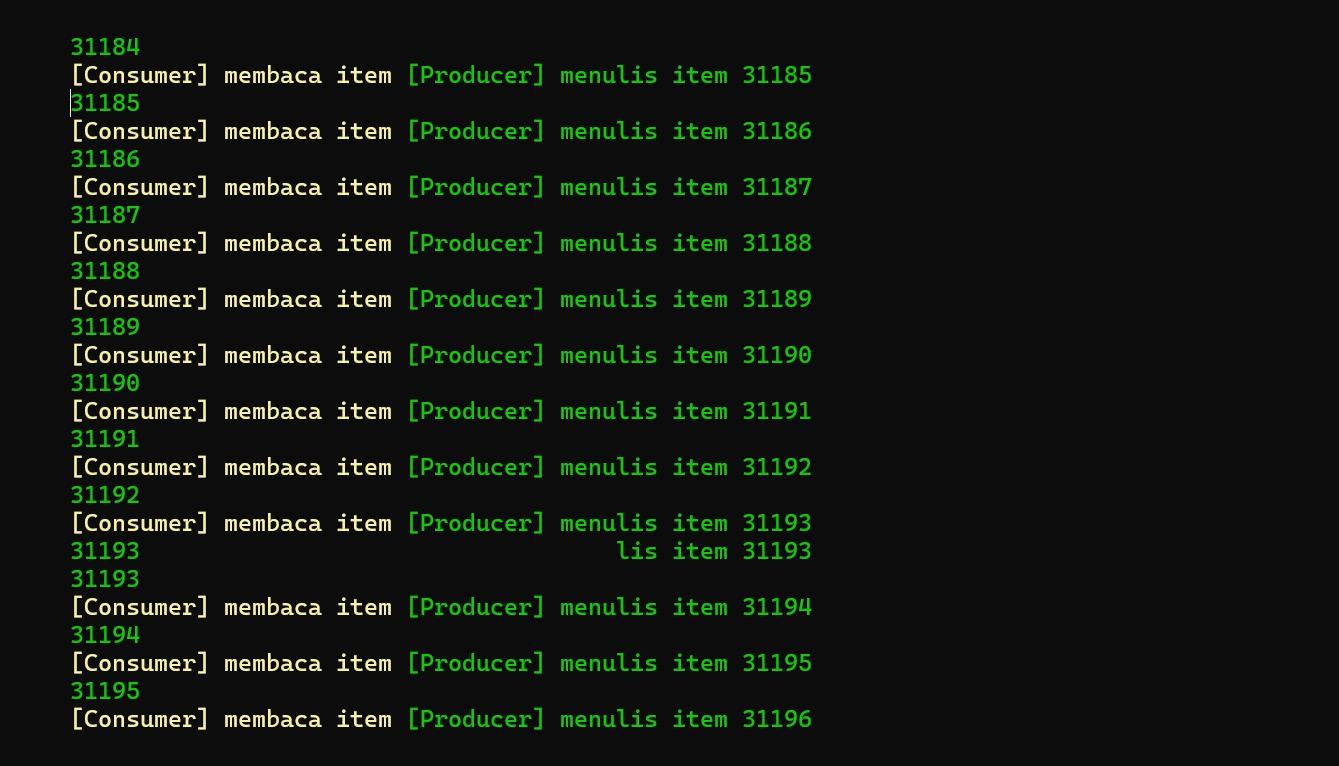
\includegraphics[width=0.85\textwidth]{Figure/09/1.jpeg}
    \caption{Contoh output QEMU yang menunjukkan \textit{race condition} pada Producer-Consumer tanpa sinkronisasi.
             Perhatikan baris yang terpotong dan angka yang tidak konsisten.}
    \label{fig:m09-sesi1}
\end{figure}
